\chapter{Discussion, Conclusion and Future Work}\label{Ch:discussion}

\section{Discussion}
We now discuss possible interpretations of our results as well as their limitations and sources of possible bias. One fundamental concern relates to our own ``synthetic'' dataset and its representation of the actual graphics corruptions that occur during gameplay. First, our approach in developing the \texttt{Glitchify} program consisted of classifying artifacts into categories based on their appearance, however, the viability of this procedure is debatable. Whereas the structure and design of screen-tearing and stuttering were sufficiently understood and formally expressed, our definition of shader/shapes and line pixelation artifacts might be too narrow to capture all of the variations of these corruptions seen in reality. This discrepancy might be responsible for some bias present in our artificial dataset, which in turn affects all further results.\\\hspace{\fill}\\
Another data-related concern comes from the frames we extracted from games to feed into \texttt{Glitchify}. We require that all these frames are normal, i.e. do no contain any corruptions. In order to ensure this holds, we manually processed collected images in an attempt to perform a first-order quality check. Due to surrealistic contents of most games, working with individual frames rather that a continuous gameplay makes it harder, if not impossible, to correctly discriminate between unwanted artifacts and intentional design. Figure \ref{confused} displays examples of such images.
\begin{figure}[H]
\centering
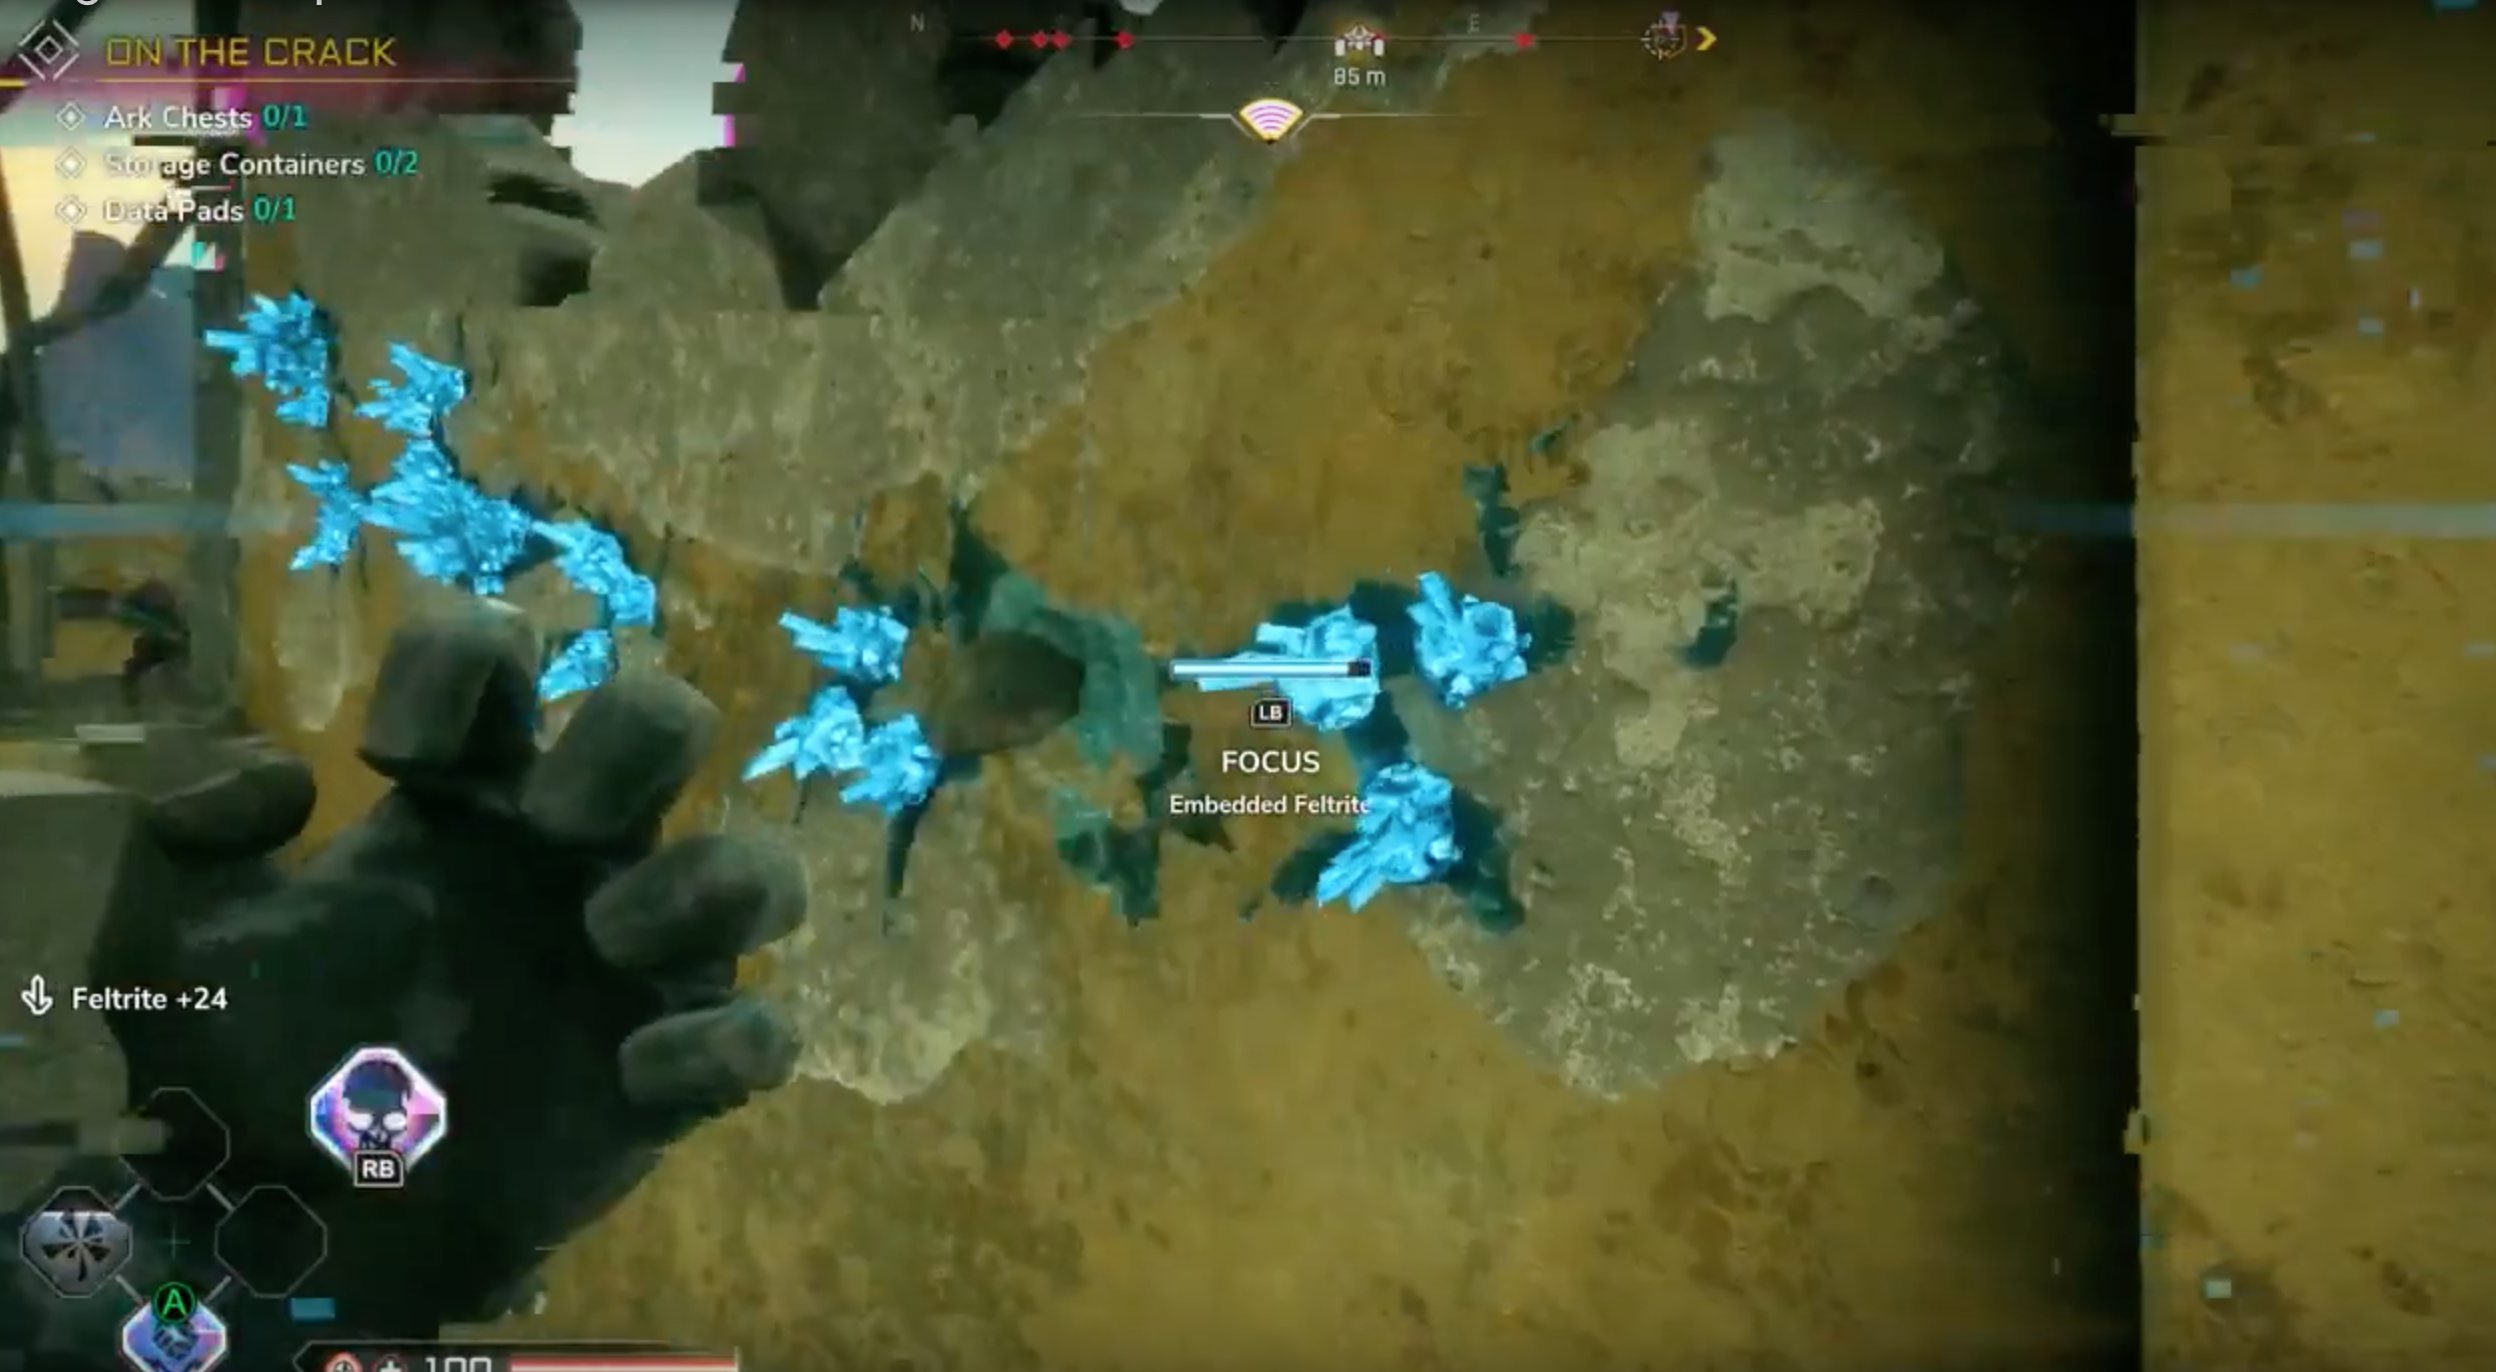
\includegraphics[scale=0.18]{images/corr2.png}
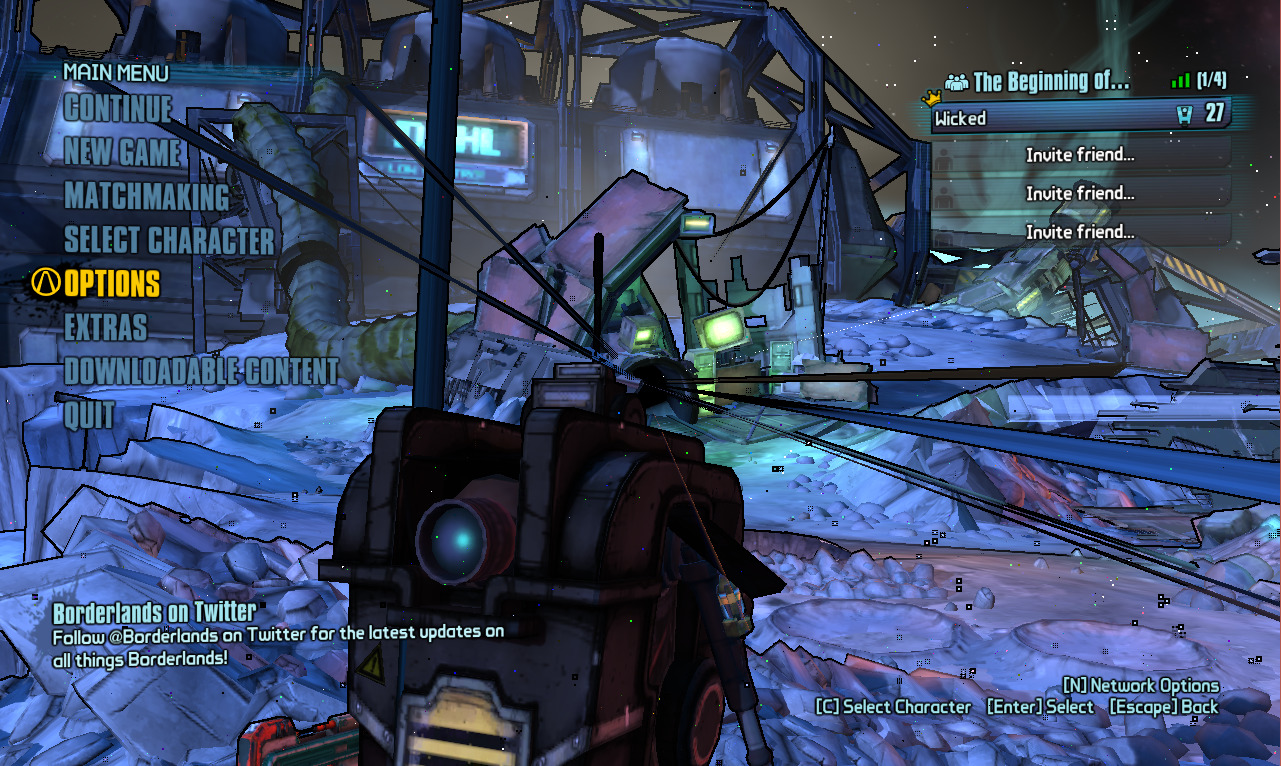
\includegraphics[scale=0.16]{images/shape3.jpg}\\[2ex]
\caption{A normal (left) and a corrupted (right) images.}
\label{confused}
\end{figure}

%%%%%%%%%%%%%%%%%%%%
\newpage
%%%%%%%%%%%%%%%%%%%%%
\noindent
Regarding the individual models, the accuracy on the test set drops from training stage 1 (Table \ref{tab:models}) to training stage 2 (Table \ref{tab:stage2}). This is mostly due to the fact the models in training stage 2 have never seen the games they are being tested on. In this project, however, the recall rate is the most important metric to consider as it is crucial to make sure that during gameplay, we detect as my corrupted images as possible so we can fix them. In training stage 2, we can see that most models produce good recalls on games they have never seen, showing a good degree of generalizability. The artifacts comprising Discoloration and Screen Tearing have very low recall scores in training stage 2 (0.66 and 0.5 respectively) versus 0.95 and 0.80 in training stage 1, demonstrating that those models overfit the training data and are not generalizable to new games. We speculate that the low accuracy score we have obtained on the heldout test set is due to the ``glitchy" look of one of the games we have included in data set C (Crackdown 3). Both images in Figure \ref{fig:hard} are from this game. Additionally, there are a lot of explosions that happened during the gameplay, and we suspect that the frames we labeled as ``normal" are not entirely normal.\\

\begin{figure}[h]
    \centering
    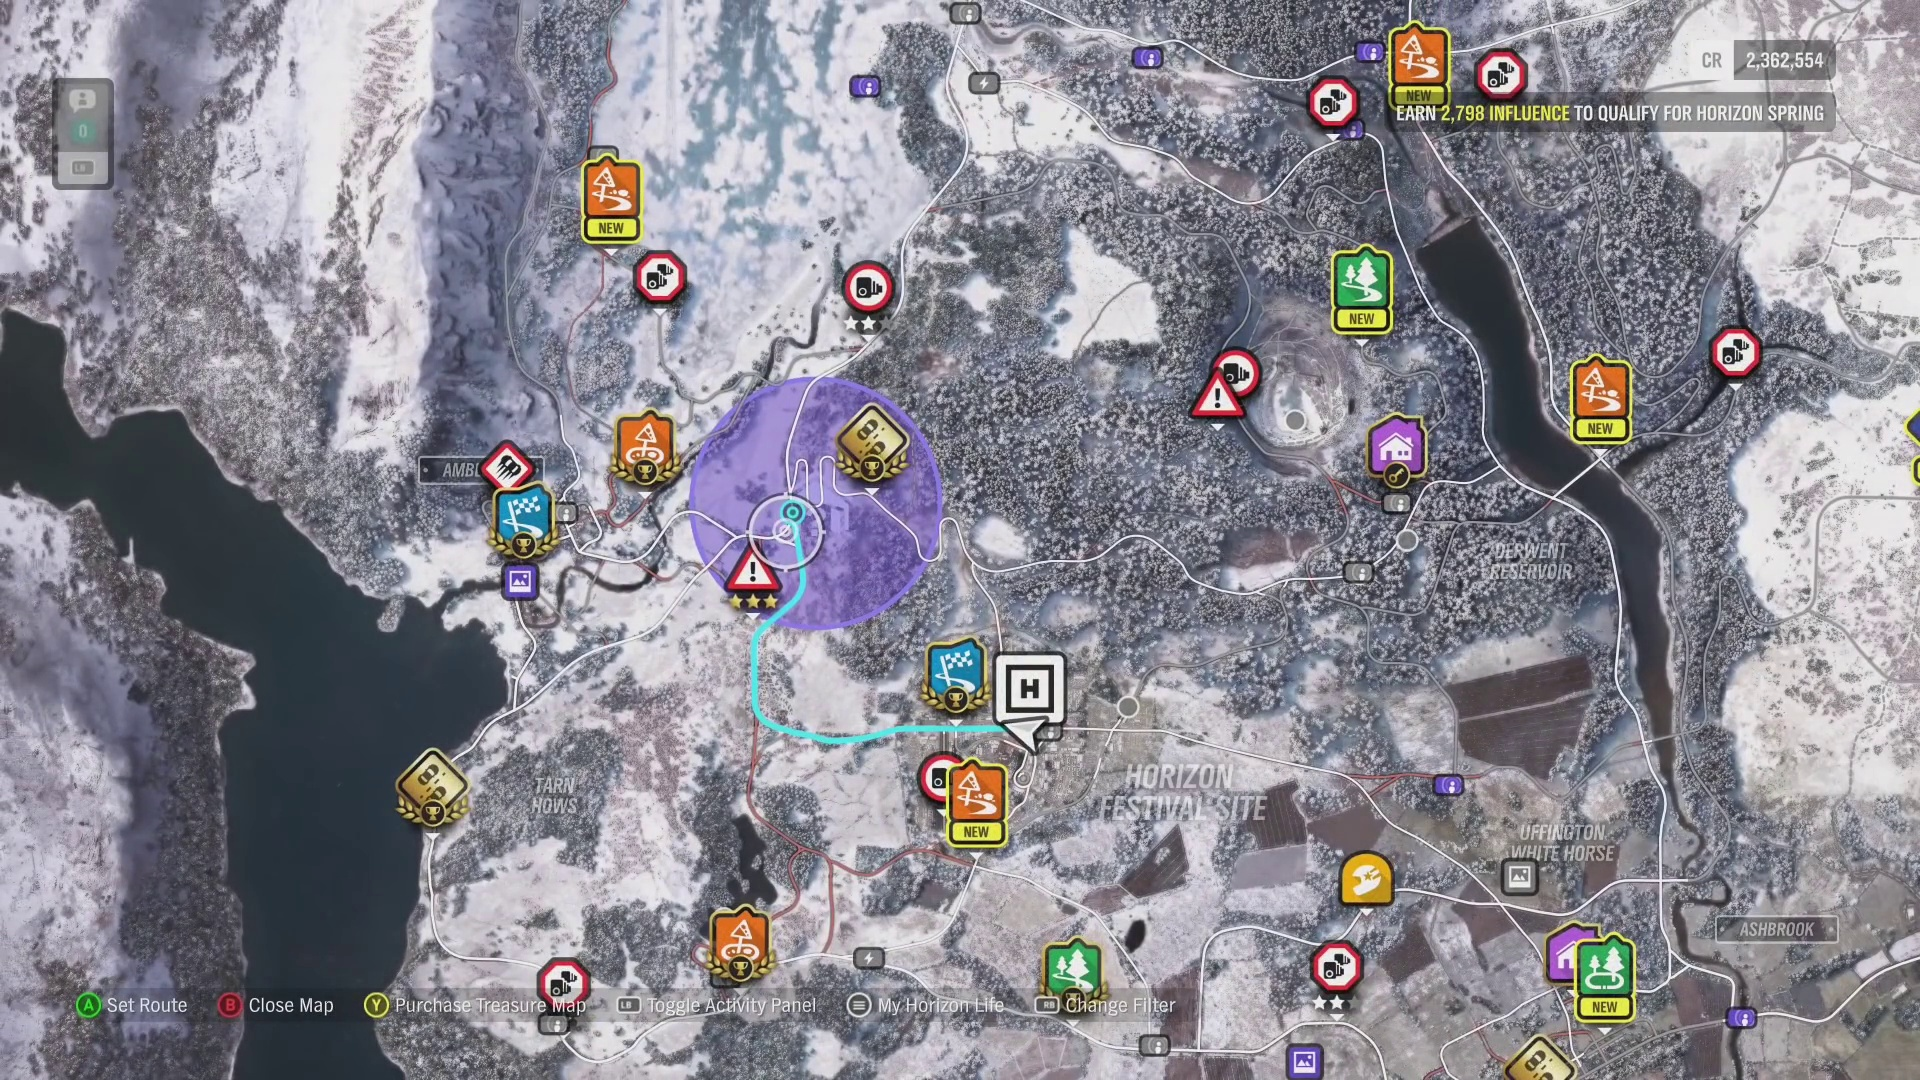
\includegraphics[scale=0.11]{images/discoloration_146.jpg}
    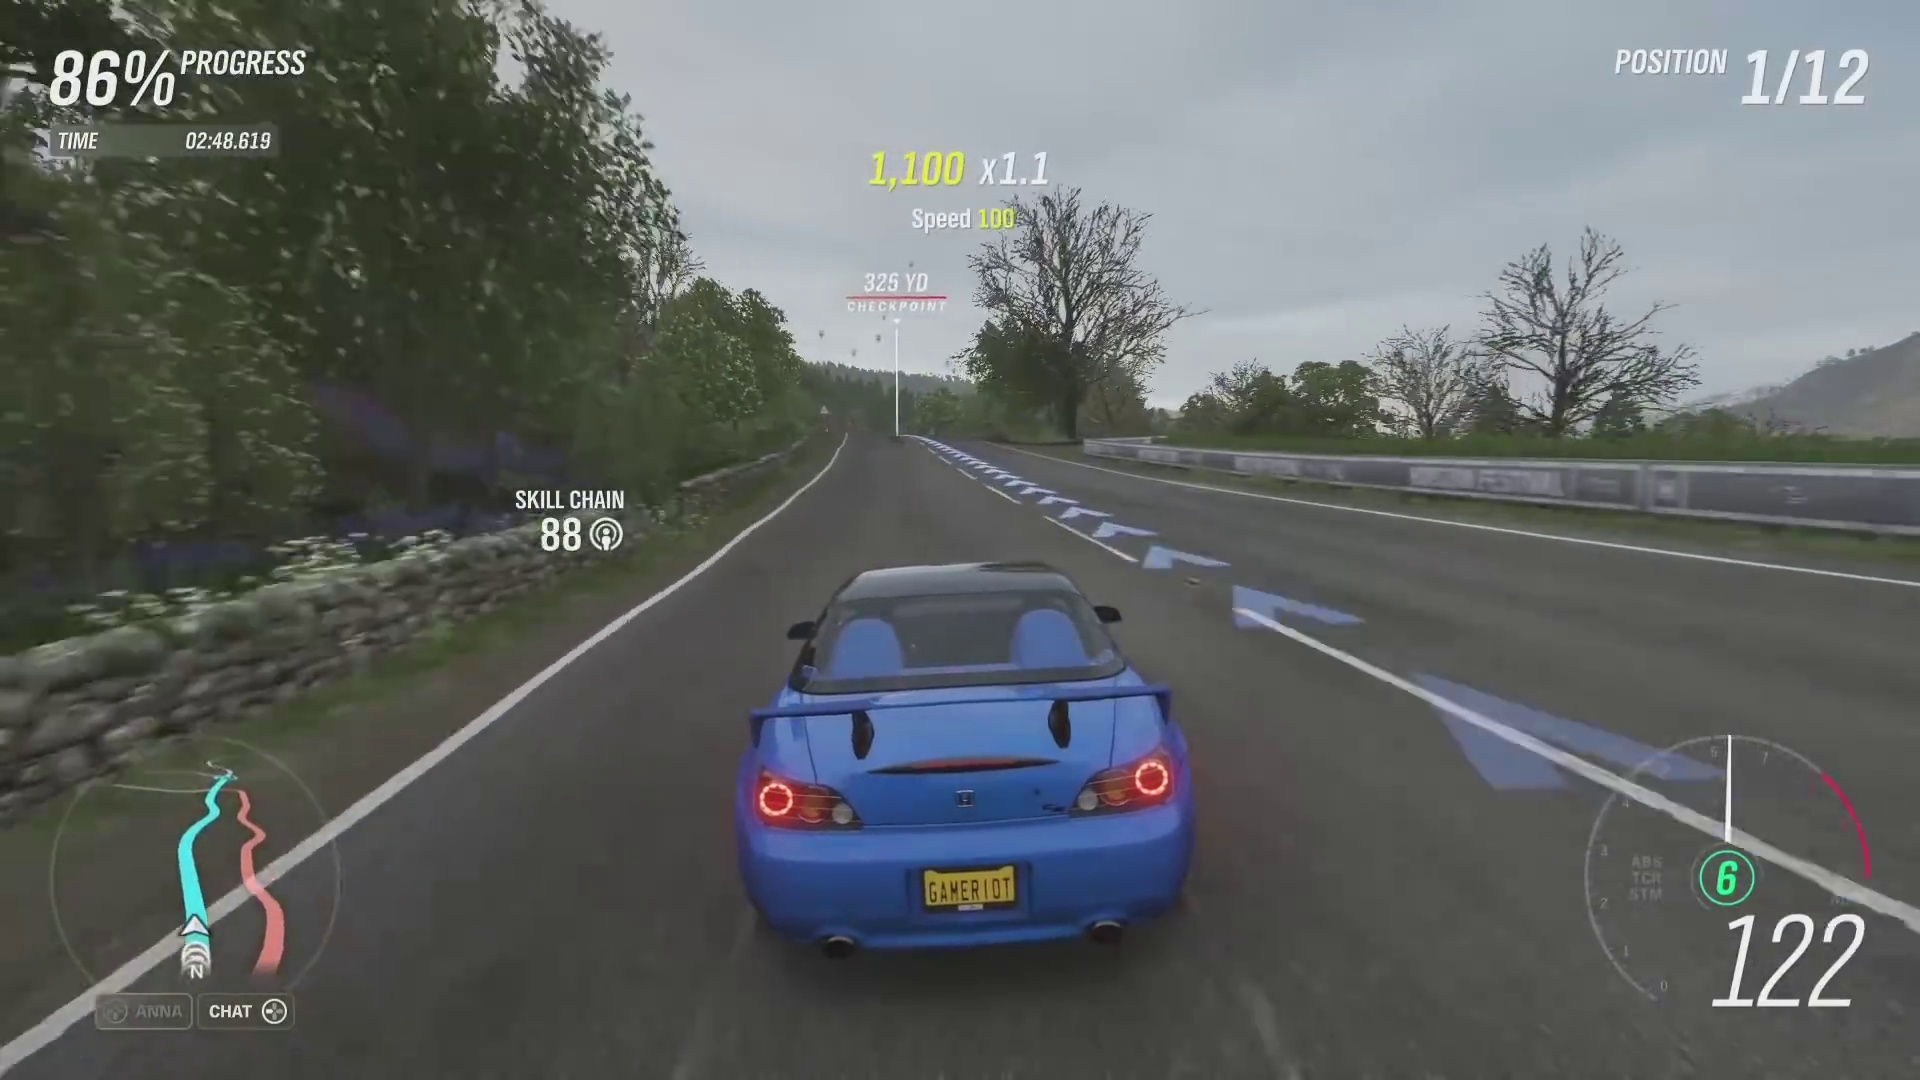
\includegraphics[scale=0.11]{images/dotted_line_345.jpg}
    
\includegraphics[scale=0.11]{images/shader_1.jpg}
    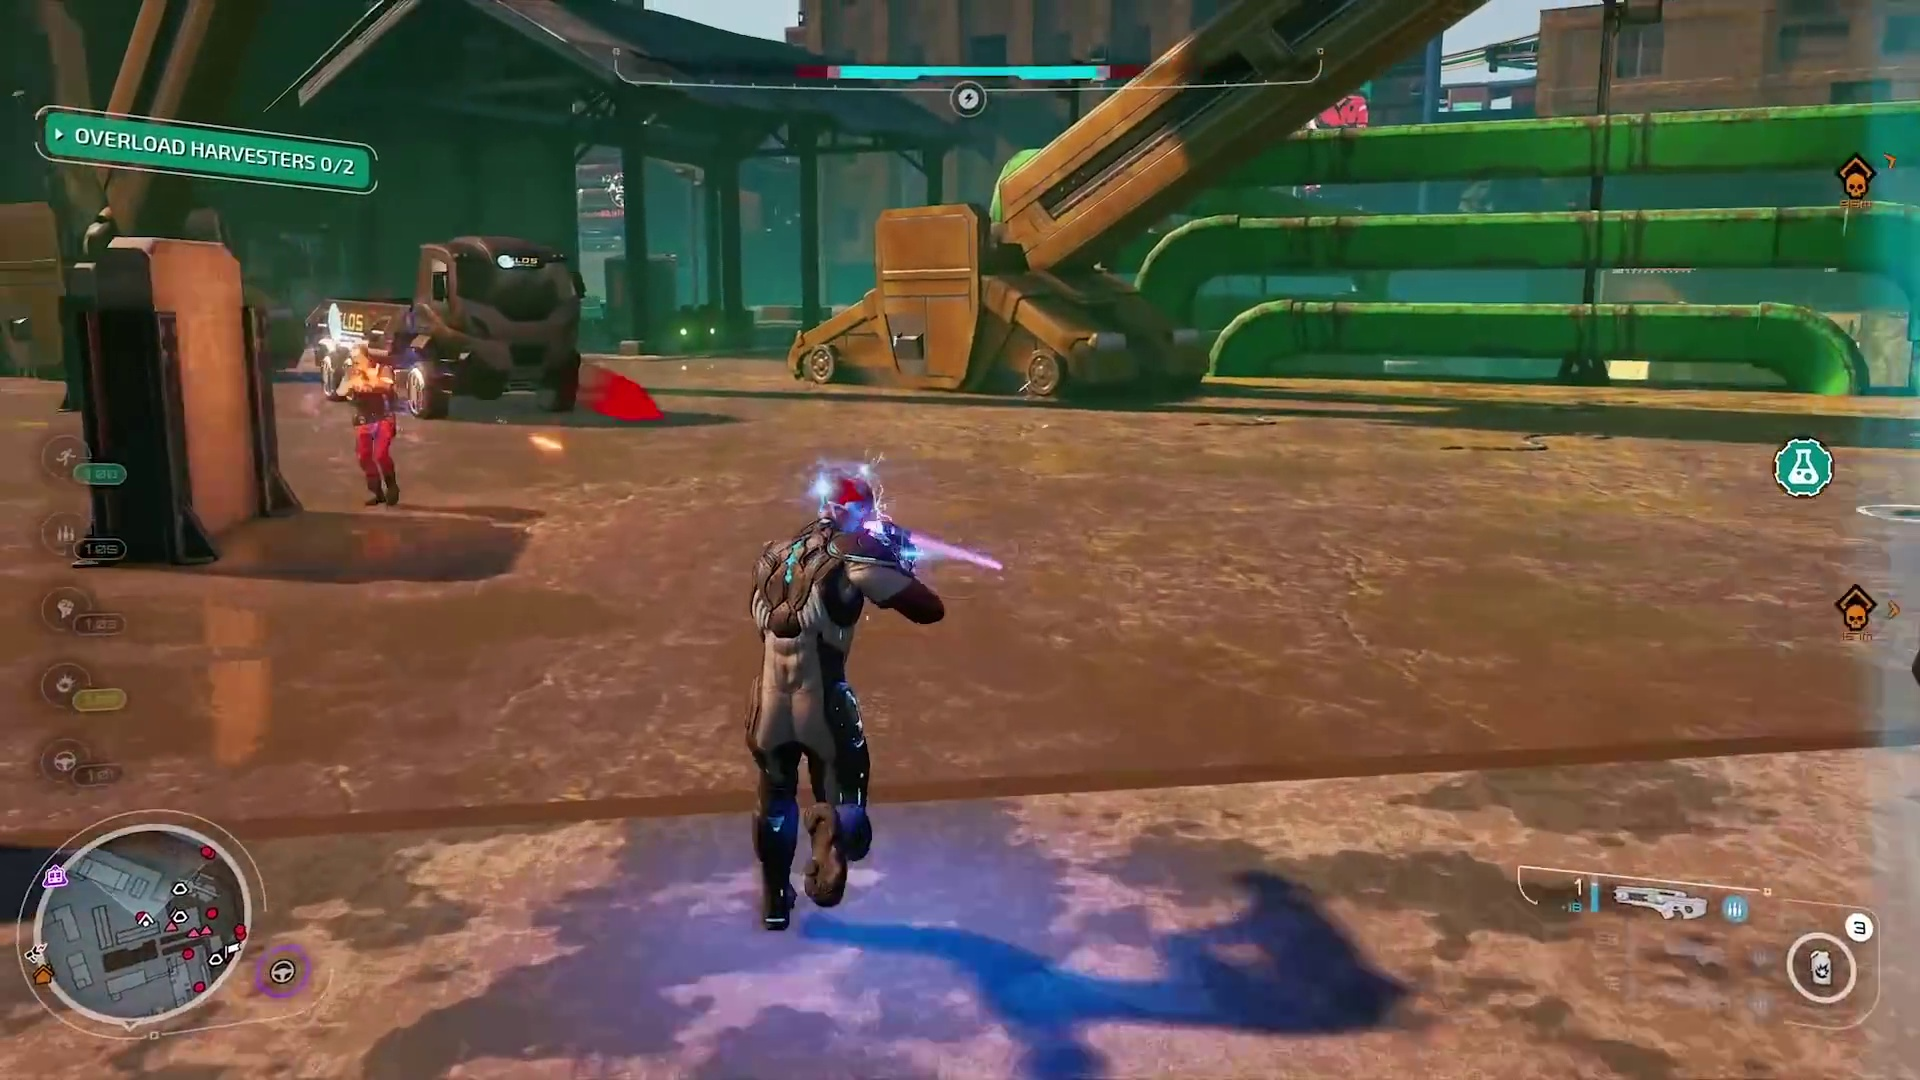
\includegraphics[scale=0.11]{images/screen_tearing_132.jpg}
    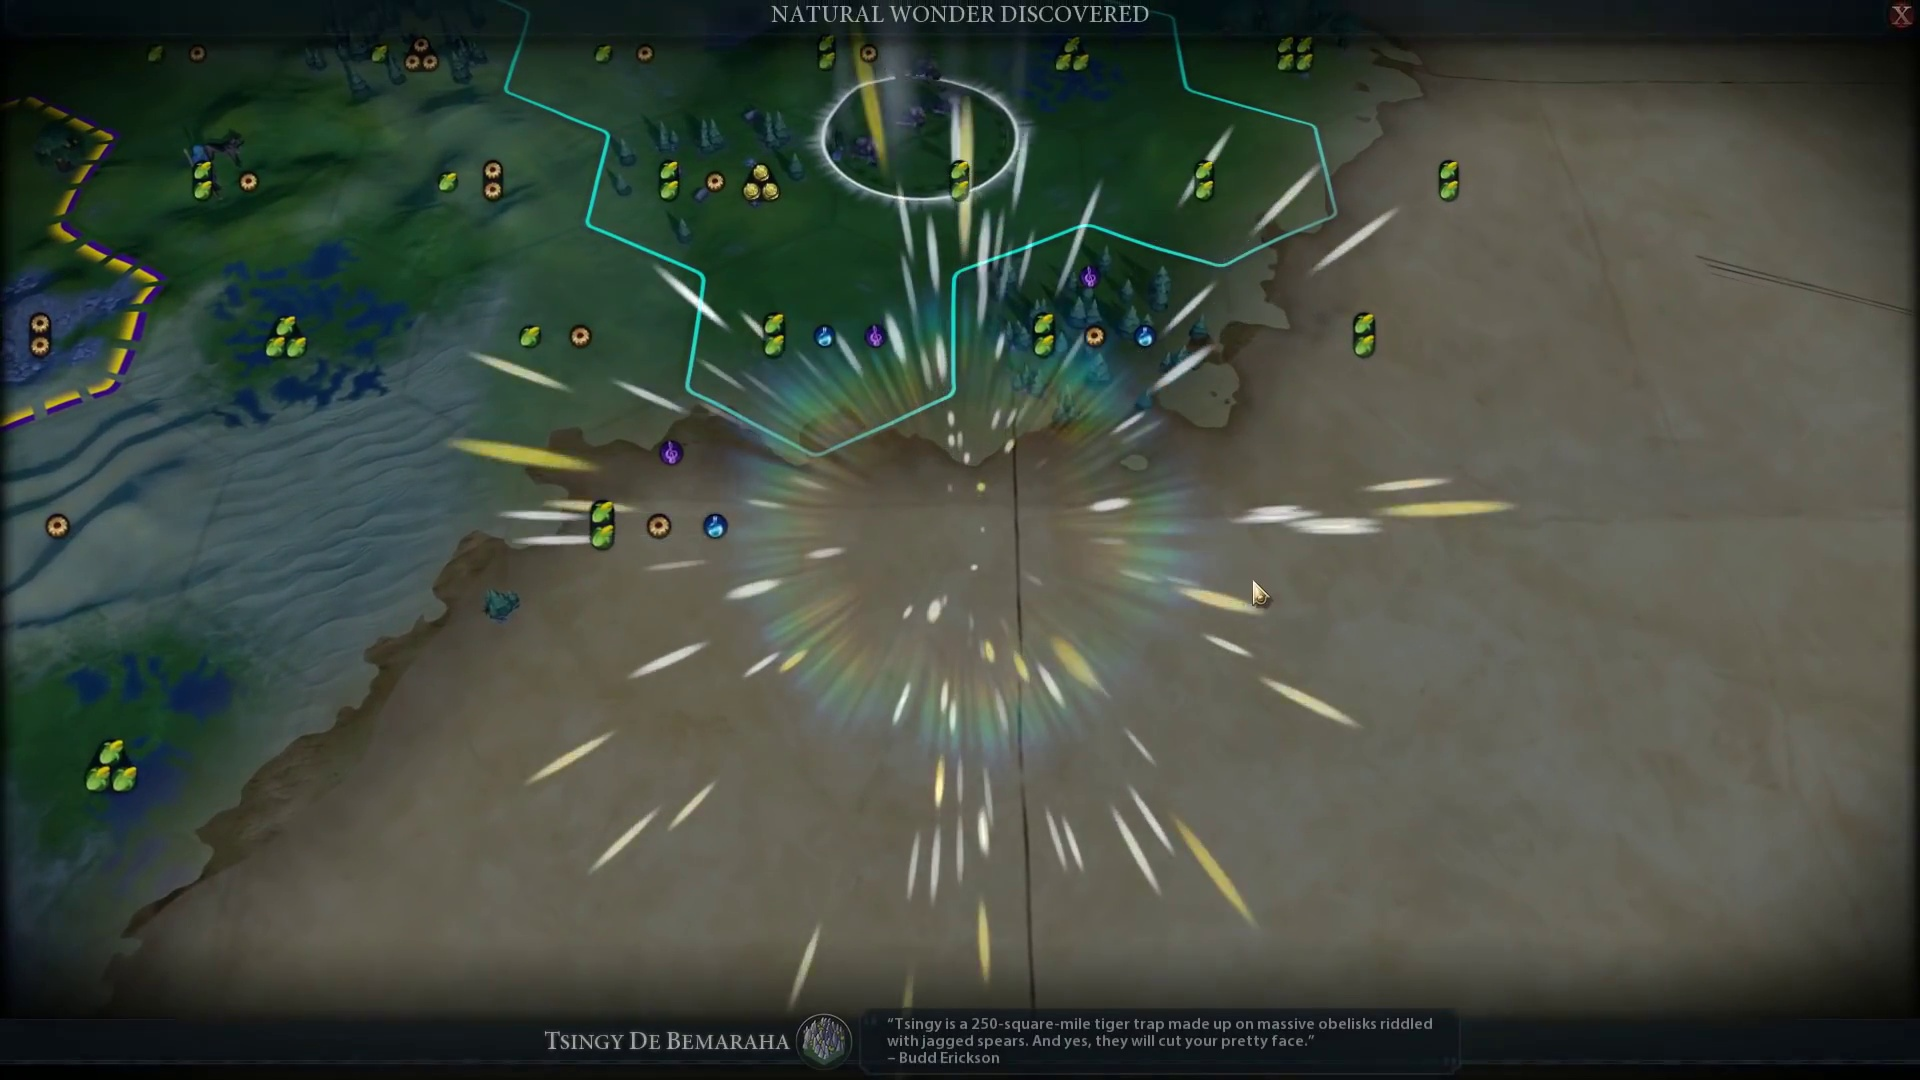
\includegraphics[scale=0.11]{images/shape_56.jpg}
    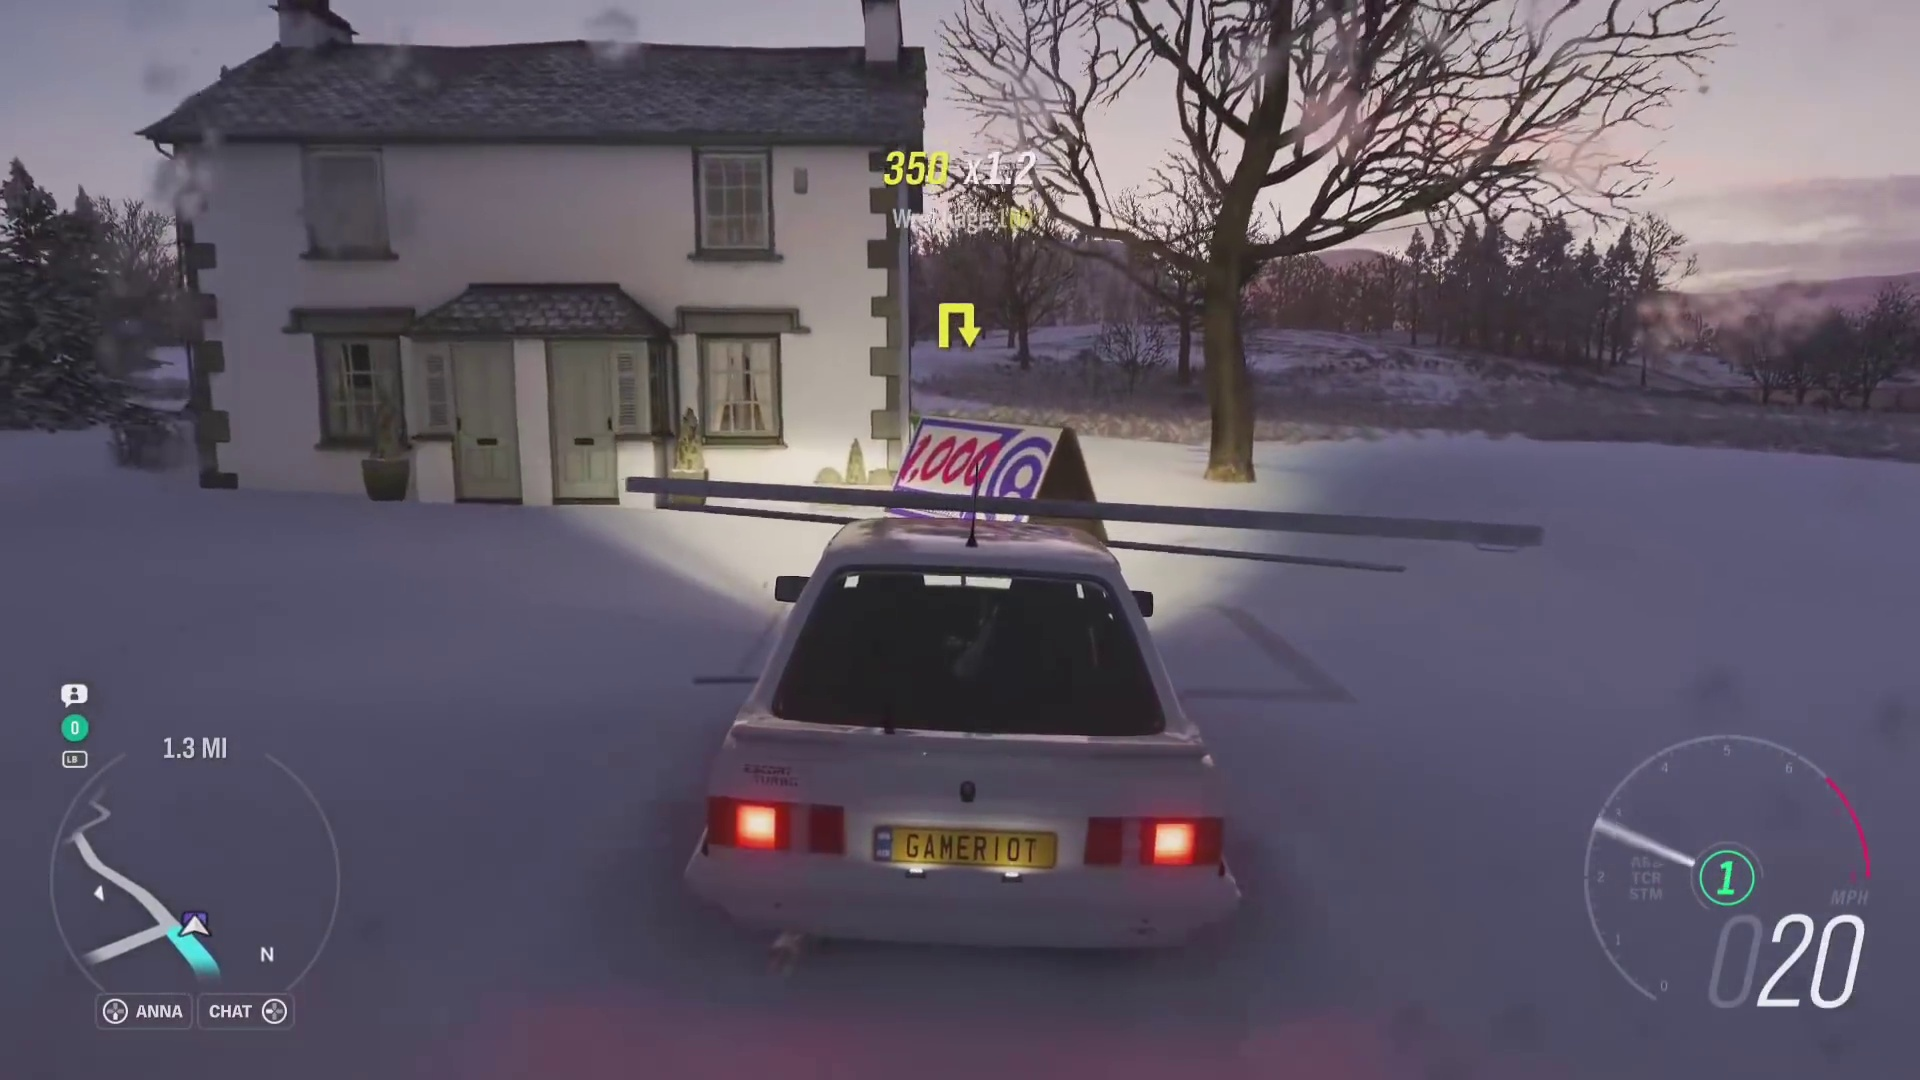
\includegraphics[scale=0.11]{images/shape_91.jpg}
    \caption[Visualization of False Positives]{Visualization of False Positives. On the left, from top to bottom the normal images are misclassified as discoloration, shader, shape. On the right, from top to bottom the images are misclassified as dotted line, screen tearing, shape.}
    \label{fig:FP}
\end{figure}



\noindent Another metric that we consider which is less important than recall is precision. Precision is the ratio of corrupted images over the images that were predicted to be corrupted. A low precision corresponds to a high number of false positives. In Table \ref{tab:stage2}, we can see that most models produce a large number of false positives. This means that these models are conservative and label a lot of normal images as corrupted. After looking at Figure \ref{fig:FP} we can see that some games truly look like they have an artifact, and until the models see those games and learn what is ``normal", it is expected for them to produce a lot of false positives.\\

%\noindent There are some limitations and biases associated with how we conducted the data generation. First and foremost, the images we extracted from videos may have already contained artifacts (i.e texture pop-in) due to compression. Also, some frames may look ``glitchy” but they are actually not. Examples of this are in Figure \ref{fig:FP} where models missclassified normal images as corrupted. We did go through the images manually to make sure that they do not already contain glitches, but did not perform the manual vetting exhaustively over the whole dataset. \\

%\noindent Second, when extracting images from gameplays on YouTube\texttrademark, even though some videos covered the entire gameplay, a number of them only covered one or a few chapters of the game. This means that not all environments/states in that game were represented which restricts the scope of our data. This could potentially lead to our model being less robust. Additionally, screen tearing artifacts that are produced from static games can be very hard to detect, if not impossible. This leads to inaccurate labels which make it difficult for the model to converge. \\ 

%\noindent Another source of bias in our data is the pace of the game. If the game is dynamic (i.e action adventure games) where the scene is constantly changing, then sampling frames at even a high rate will result in images that are independent. On the other hand, if the game is slowly changing (i.e strategy games), then sampled frames can look very similar. This could introduce large amounts of bias in the results of the model if the images in the test set are close to those in the training set. Another existing limitation is the fact that we resize the images before feeding them to most  models. By resizing the images we lose some potentially useful information which can also reduce the strength of the rendered artifacts. 
\noindent
\\
\\
\noindent
Finally, the challenge is to find models that best perform the task of classification. Due to time limits, we were unable to try all the deep-learning models due to the long training time the tedious fine tuning that they require. Nevertheless, we have found that some traditional machine learning models that are frequently used as classifiers and take less time to train - such as logistic regression- can handle the artifact detection task well. Using the dimension-reduced features of the images as inputs, we constructed a number of machine learning models as individual glitch classifiers and selected the best models with the highest accuracy for each glitch. Our ensemble model combined all the best individual classifiers, but some models which had relatively poor performance (for example, the model used to detect little square patches) caused a lot of false positives and negatives. Since the square patch glitches were not always visible to humans, we have excluded those images with square patches from both the training sets and the testing sets. Yet the detection of the less obvious glitches might still be worth thinking about in the future.



\section{Conclusion}
In this study, we developed a software that automatically detects graphics corruptions in frames from video games. Based on a sample of screen corruption examples provided by AMD, 13 most common content-unrelated artifacts were selected, described and then recreated with a \texttt{Glitchify} program. With help of \texttt{Glitchify}, a dataset of 50,000 images was created by adding 13 different types of artifacts to normal frames extracted from 34 modern video games. Each of the 13 corruptions was learned by different models including Logistic Regression, Support Vector Machine and Linear Discriminant Analysis. The output probabilities of these individual classifiers were used for training a mixed experts Logistic Regression model intended to carry out the final classification decision. The overall accuracy on the \texttt{Glitchify}-produced test set based on games unseen during training is 69\%. 


\section{Future Work}
One promising way we can improve our results is tiling. That is, instead of resizing the images which could lead to loss of information, we break the image down into ``tiles" and treat each tile as a single image. This would require us to have knowledge about where in the image the artifacts have been inserted, so we can label the tiles appropriately. Although tiling might lead to loss of context, it could still improve our performance since we are not resizing the images.\\
Another possibility in improving our work is to conduct a finer hyper parameter grid search to train our CNN.\\

% In the future, we would like to train our model on more images, and include more games in our testing set to better evaluate the generalizability of our models. Also, we may explore more ways to represent the features and more machine-learning approaches to do the classification task. A finer grid-search of the hyper-parameters of some models can also be done to improve the performance of the models. Finally, we could search for other methods to better combine the results from individual classifiers and improve the ensemble model. \\
\noindent Since our model currently only focuses on binary classification (glitched or normal), building a multi-class classifier which outputs the type of the detected glitch would be very ideal. Since the ensemble is composed of individual models each of which are capable to detecting a specific type of glitch, the multi-class classification is feasible. \\

\noindent Another future direction is to implement real-time detection. Real-time detection would require a software that is capable of flagging each and every frame as ``normal" or ``corrupted" at a very high rate and with a high accuracy. We foresee that once a video game console is capable of achieving this, not only can it send a report of that glitch to the corresponding company, but maybe it will be also able to rectify the corrupted image before it is displayed to the user.



\endinput
